\id{IRSTI 20.01.45}{}

{\bfseries ANALYZING E-LEARNING STUDENT PERFORMANCE AND FEATURE}

{\bfseries IMPACT USING XGBOOST AND SHAP}

{\bfseries M.
Madeniyetov}
\begin{figure}[H]
	\centering
	
\includegraphics[width=0.8\textwidth]{media/ict/image16}
	\caption*{}
\end{figure}


\emph{Kazakh-British Technical University, Almaty, Kazakhstan}

{\bfseries \textsuperscript{\envelope }}Corresponding author: madeniyetov@kbtu.kz

E-learning has become an essential part of modern education, providing
flexibility and accessibility to students worldwide. However,
understanding the factors that influence student success in online
learning remains a challenge. In this study, we analyze student
performance in e-learning courses using the XGBoost classifier and SHAP
(SHapley Additive exPlanations) to identify key features that impact
academic outcomes. The dataset, obtained from the UC Irvine Machine
Learning Repository, contains student information related to personal
background, family environment, and educational habits. We categorize
student performance in three ways: predicting exact grades, classifying
students as pass/fail, and determining whether they achieve good or not
good grades. Our findings show that certain features significantly
influence student performance. For pass/fail prediction, factors such as
last semester's GPA, expected graduation GPA, and parental education
levels were among the most impactful. In contrast, for good/not good
classification, features like course ID, having a job, and accommodation
type played a major role. The prediction results show that the model
performs best in pass/fail classification, achieving an accuracy of
97.43\%, while good/not good classification reached 80.07\%. This
suggests that predicting broad categories like pass/fail is much easier
than predicting exact grades. These findings highlight the importance of
carefully selecting features when analyzing student performance. Future
research could expand this study by using a larger and more diverse
dataset, incorporating additional features such as student engagement
metrics, online activity logs, and psychological factors.

{\bfseries Keywords:} E-learning, Student performance, Machine learning,
XGBoost, SHAP (SHapley Additive exPlanations), Predictive modeling,
Online education.

{\bfseries XGBOOST ЖӘНЕ SHAP КӨМЕГІМЕН E-LEARNING СТУДЕНТТЕРІНІҢ}

{\bfseries ӨНІМДІЛІГІ МЕН МҮМКІНДІК ӘСЕРІН ТАЛДАУ}

{\bfseries M.Mәдениетов}

\emph{Қазақ-Британ техникалық университеті, Алматы, Қазақстан,}

\emph{e-mail:madeniyetov@kbtu.kz}

E-learning бүкіл әлем бойынша студенттерге икемділік пен қолжетімділікті
қамтамасыз ететін заманауи білім берудің ажырамас бөлігіне айналды.
Дегенмен, онлайн оқудағы оқушылардың үлгеріміне әсер ететін факторларды
түсіну қиын болып қала береді. Бұл зерттеуде біз академиялық нәтижелерге
әсер ететін негізгі сипаттамаларды анықтау үшін XGBoost классификаторы
мен SHAP (SHapley Additive Explanations) көмегімен электрондық оқыту
курстарындағы студенттердің жұмысын талдаймыз. Калифорния
университетінен, Ирвиннің машиналық оқыту репозиторийінен алынған
деректер жинағы студенттердің жеке тәжірибесіне, отбасылық тарихына және
оқу әдеттеріне қатысты ақпаратты қамтиды. Студенттердің үлгерімін үш
жолмен жіктейміз: нақты бағаларды болжау, оқушыларды сәтті/өтпеген деп
жіктеу және олардың жақсы немесе нашар баға алатынын анықтау. Біздің
нәтижелеріміз белгілі бір сипаттамалардың оқушылардың оқу үлгеріміне
айтарлықтай әсер ететінін көрсетеді. Өту/өтпеу нәтижелерін болжауда
соңғы семестрдегі GPA, бітіру кезіндегі күтілетін GPA және ата-аналардың
білім деңгейі сияқты факторлар ең ықпал етті. Керісінше, жақсы/жаман
жіктеу үшін курс идентификаторы, жұмыстың қолжетімділігі және
орналастыру түрі сияқты сипаттамалар маңызды рөл атқарды. Болжау
нәтижелері үлгінің 97,43\% дәлдікке, ал жақсы/жаман классификацияға
80,07\% қол жеткізіп, өту/сәтсіз жіктеуде ең жақсы орындайтынын
көрсетеді. Бұл өту/өтпеген сияқты кең санаттарды болжау нақты бағаларды
болжаудан әлдеқайда оңай екенін көрсетеді. Бұл нәтижелер оқушының
жұмысын талдау кезінде мүмкіндіктерді мұқият таңдаудың маңыздылығын
көрсетеді. Болашақ зерттеулер бұл зерттеуді үлкенірек және әртүрлі
деректер жиынтығын, соның ішінде студенттердің қатысу жылдамдығы,
желідегі белсенділік журналдары және психологиялық факторлар сияқты
қосымша шараларды пайдалана отырып кеңейтуі мүмкін.

{\bfseries Түйiн сөздер:} E-learning, студенттердің өнімділігі, машиналық
оқыту, XGBoost, SHAP (Shapley Additive Explainers), болжамды модельдеу,
онлайн білім беру.

{\bfseries АНАЛИЗ УСПЕВАЕМОСТИ СТУДЕНТОВ ЭЛЕКТРОННОГО ОБУЧЕНИЯ}

{\bfseries И ВЛИЯНИЯ ФУНКЦИЙ С ИСПОЛЬЗОВАНИЕМ XGBOOST И SHAP}

{\bfseries M. Mәдениетов}

\emph{Казахстанско-Британский технический университет, Алматы,
Казахстан,}

\emph{e-mail:madeniyetov@kbtu.kz}

Электронное обучение стало неотъемлемой частью современного образования,
обеспечивая гибкость и доступность для студентов по всему миру. Однако
понимание факторов, влияющих на успеваемость студентов в
онлайн-обучении, остается сложной задачей. В этом исследовании мы
анализируем успеваемость студентов на курсах электронного обучения с
помощью классификатора XGBoost и SHAP (SHapley Additive exPlanations)
для выявления ключевых характеристик, влияющих на академические
результаты. Набор данных, полученный из репозитория машинного обучения
Калифорнийского университета в Ирвайне, содержит информацию об учащихся,
связанную с личным опытом, семейной обстановкой и образовательными
привычками. Мы классифицируем успеваемость учащихся тремя способами:
прогнозирование точных оценок, классификация учащихся как сдавших/не
сдавших и определение того, получают ли они хорошие или плохие оценки.
Наши результаты показывают, что определенные характеристики существенно
влияют на успеваемость учащихся. Для прогнозирования сдавших/не сдавших
такие факторы, как средний балл за последний семестр, ожидаемый средний
балл по окончании обучения и уровень образования родителей, были одними
из самых влиятельных. Напротив, для классификации «хорошо/плохо» такие
характеристики, как идентификатор курса, наличие работы и тип
размещения, играли важную роль. Результаты прогнозирования показывают,
что модель лучше всего работает в классификации сдал/не сдал, достигая
точности 97,43\%, а классификация хорошо/не хорошо достигла 80,07\%. Это
говорит о том, что прогнозирование широких категорий, таких как сдал/не
сдал, намного проще, чем прогнозирование точных оценок. Эти результаты
подчеркивают важность тщательного выбора признаков при анализе
успеваемости учащихся. Будущие исследования могут расширить это
исследование, используя более крупный и разнообразный набор данных,
включив дополнительные признаки, такие как показатели вовлеченности
учащихся, журналы онлайн-активности и психологические факторы.

{\bfseries Ключевые слова:} Электронное обучение, успеваемость студентов,
машинное обучение, XGBoost, SHAP (аддитивные объяснения Шепли),
прогностическое моделирование, онлайн-образование.

{\bfseries Introduction.} In today' s digital world,
e-learning systems provide many benefits to both students and
organizations. The main advantages of e-learning is the ability to allow
flexibility and accessibility. Students can learn at their own pace,
anytime and anywhere, making education more convenient for those with
busy schedules or limited access to traditional classrooms {[}1{]}. This
flexibility is especially valuable for working professionals, as well as
students from different regions and backgrounds who may not have the
opportunity to attend in-person classes {[}2{]}. E-learning also
promotes the use of modern technologies to enhance learning. For
example, interactive features such as multimedia, virtual discussions,
and real-time feedback make learning more engaging {[}3{]}. Many
students find these technologies helpful for communication and
collaboration, especially through social networking platforms {[}1{]}.
In addition, e-learning encourages students to become more independent
learners by giving them access to a wide range of online resources and
learning materials {[}4{]}. From an organization' s point
of view, e-learning shows strategic advantages. Research shows that when
businesses and governments adopt integrated e-learning strategies, they
often achieve better results compared to focusing only on content
delivery {[}5{]}.

Successful e-learning systems can improve employee skills, support
lifelong learning, and contribute to the overall development of
societies and economies {[}5{]}, {[}2{]}. Furthermore, e-learning can
help reduce educational costs and improve the efficiency of training
programs {[}3, 4{]}.

\emph{{\bfseries Problem statement}}

Despite these benefits, it is important to carefully design e-learning
programs to ensure that they meet the needs of students and
organizations. In this study, we focus on identifying the
characteristics of the design and content of the e-learning course that
are important to students to successfully complete the course.

\emph{{\bfseries Related work}}

To ensure that students complete their courses successfully,
understanding the characteristics that contribute to the effectiveness
of e-learning is essential. Several studies have explored the key
factors that influence student performance and satisfaction in
e-learning.

Technological factors play an important role in the success of
e-learning systems. The quality of information technology
infrastructure, system usability, and the availability of reliable
internet services are critical for course completion {[}6, 7{]}. For
instance, low-quality internet services could reduce learning progress,
especially in regions with limited technical support {[}7{]}.

Additionally, systems that are easy to navigate and provide
well-structured content lead to higher satisfaction and better
performance outcomes {[}8{]}.

Instructor and learner qualities also influence e-learning success.
Instructors' technical skills and attitudes toward e-learning impact how
effectively students engage with the system {[}9,10{]}. Similarly,
students with strong self-regulation, time management, and emotional
intelligence are more likely to complete courses successfully {[}11{]}.
Self-regulated learners tend to plan, organize, and stay motivated,
which helps them manage the flexibility and challenges of online
learning {[}11{]}.

Collaboration and interaction features are important for maintaining
student engagement and satisfaction {[}8, 12{]}. E-learning platforms
that promote interaction and collaboration with peers strengthen a sense
of community, reducing feelings of isolation. An effective learning
design such as mixed learning approaches improves student achievement by
integrating online and offline activities {[}12, 9{]}.

However, despite these benefits, challenges remain. Issues such as
technical support, financial constraints, and change management could
create difficulties when implementing e-learning {[}9{]}. Instructors
and institutions need to be adequately prepared and supported to ensure
a smooth e-learning experience. Additionally, the availability of
diverse and high-quality course content is necessary for student
satisfaction and learning success {[}8,10{]}.

Successful course completion in e-learning depends on multiple
interconnected factors, including technology infrastructure, instructor
and learner capabilities, and collaborative features. Addressing these
elements and overcoming related challenges is crucial for enhancing the
effectiveness of e-learning systems.

{\bfseries Materials and methods.} This section consists of three steps:
(1) describing the dataset, (2) analyzing the prediction, and (3)
calculating the prediction, as shown in Figure 1.


\begin{figure}[H]
	\centering
	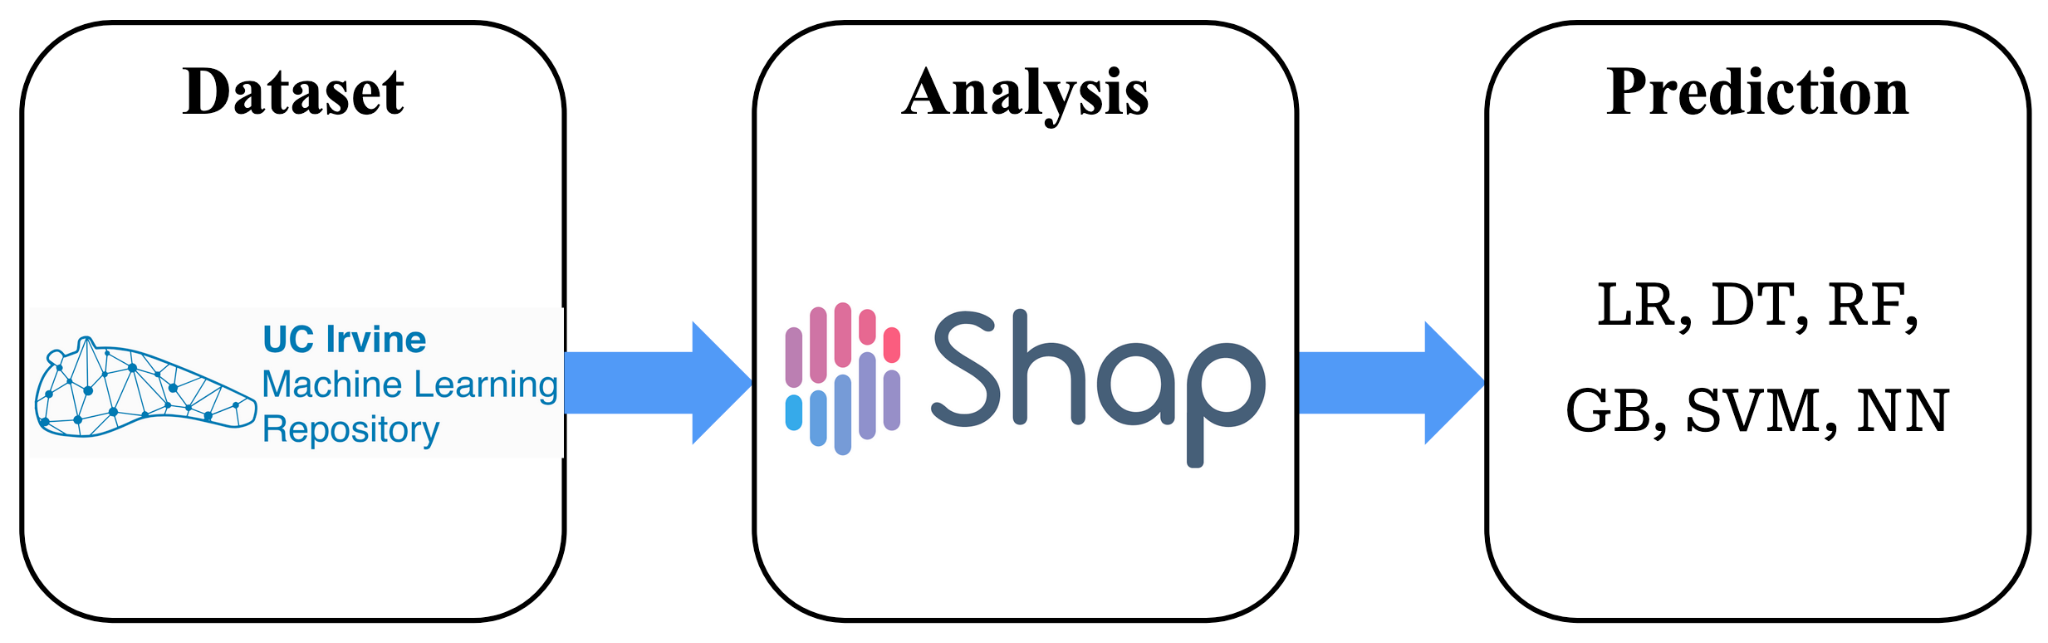
\includegraphics[width=0.8\textwidth]{media/ict/image17}
	\caption*{}
\end{figure}


{\bfseries Fig.1- An overview of the research methodology}

\emph{{\bfseries Dataset Description}}

E-Learning student dataset from UC Irvine Machine Learning Repository
was used for this research {[}13{]}. The dataset contains information
about students'{} end-of-term performance in the Faculty
of Engineering and the Faculty of Educational Sciences. This dataset
includes 145 students and 31 different features that cover personal
details, family background, and education habits. The dataset is
multivariate and falls under the social sciences category. The target
variable is the final course grade, which ranges from 0 (Fail) to 7 (A).
The features are divided into three groups. The First one is Personal
Information (Features 1-10) such as age, gender, high school type,
scholarship type, etc. The Second group is Family Information (Features
11-16), it covers parents'{} education, number of
siblings, marital status, and parents'{} occupations. The
third one is Educational Habits (Features 17-30), it includes study
hours, reading habits, class attendance, exam preparation style,
note-taking, listening, etc. The dataset is clean, meaning there were no
missing (null) values or duplicate records.

\emph{{\bfseries Prediction Analysis}}

In this part of our research, we used SHAP (SHapley Additive
exPlanations) to understand which features contributed the most to our
model' s predictions. SHAP helps explain how each feature
affects the final prediction, which is especially useful when working
with complex models {[}14{]}. We used the mean SHAP bar plot to find out
which features are the most important overall {[}14{]}. The plot shows
the average SHAP value for each feature. This makes it easy to see which
features have the most influence on predictions. In this research, we
identify the top 12 most important features influencing student
performance.

We begin by predicting all grades using all available features. Then, we
focus on distinguishing between passing and failing students by
converting grades into binary values. Finally, we classify students
based on high academic achievement, where only the top grades are
considered good. For each of these cases, we identify the most
influential features using SHAP (SHapley Additive exPlanations).

First, we predict all letter grades (A to F) using all features in the
dataset. A machine learning model is trained to classify student
performance into these categories. We then use SHAP to determine which
features contribute the most to grade predictions. Next, we refine our
analysis by converting grades into a binary pass/fail classification.
Here, grades A, B, C, and D are mapped to 1 (pass), while grade F is
mapped to 0 (fail). We train a machine learning model on this binary
classification task and use SHAP to extract the most important features
that determine passing or failing status. Lastly, we analyze the
characteristics of high-achieving students by classifying grades A and B
as good (1) and all other grades as not good (0). Again, we train a
machine learning model and use SHAP to identify the features that most
strongly influence high performance.

{\bfseries Table 1- Feature Extraction Cases}

%% \begin{longtable}[]{@{}
%%   >{\centering\arraybackslash}p{(\linewidth - 4\tabcolsep) * \real{0.2886}}
%%   >{\centering\arraybackslash}p{(\linewidth - 4\tabcolsep) * \real{0.3222}}
%%   >{\centering\arraybackslash}p{(\linewidth - 4\tabcolsep) * \real{0.3892}}@{}}
%% \toprule\noalign{}
%% \endhead
%% \bottomrule\noalign{}
%% \endlastfoot
%% {\bfseries Case} & {\bfseries Grade Mapping} & {\bfseries Objective} \\
%% Multi-class Grade Prediction & A, B, C, D, F as separate classes &
%% Identify top features influencing all grades \\
%% Pass/Fail Classification & A, B, C, D → 1 (Pass),
%% 
%% F → 0 (Fail) & Determine features affecting passing or failing \\
%% Good Student Classification & A, B → 1 (Good),
%% 
%% C, D, F → 0 (Not Good) & Identify features contributing to high
%% performance \\
%% \end{longtable}

\emph{Function get\_top\_features(dataset):}

\emph{X = dataset without "GRADE"}

\emph{y = "GRADE" column from dataset}

\emph{Train an XGBoost classifier using X and y}

\emph{Compute SHAP values for the model}

\emph{Calculate mean absolute SHAP values for each feature}

\emph{Sort features by SHAP importance and select the top 12}

The function starts by separating features from the target variable. It
then trains an XGBoost classifier to predict grades. SHAP values are
computed to measure the impact of each feature on the model's
predictions. By taking the mean absolute SHAP values, the most important
features are identified.

\emph{{\bfseries Prediction Calculation}}

For the prediction calculation, we used the XGBoost Classifier
(XGBClassifier) to evaluate how well the model could predict course
grades {[}15{]}. The dataset was split into training and testing sets
using an 80-20 split, meaning 80\% of the data was used for training and
20\% for testing. The top features identified from the Prediction
Analysis step were used to predict all grades, pass/fail outcomes, and
good/not-good student categories. To ensure accurate predictions,
multiple machine learning models were applied, and the model with the
highest accuracy was selected.

The models used in the analysis included Logistic Regression, Decision
Tree, Random Forest, Gradient Boosting, Support Vector Machine (SVM),
and a Neural Network (MLPClassifier). The function testAccuracy was used
to compare different models. The dataset was first split into training
and testing sets. A preprocessing pipeline was created to handle both
numerical and categorical features. Numerical features were standardized
using StandardScaler, while categorical features were transformed using
OneHotEncoder. The models were trained and evaluated using
cross-validation with five folds, ensuring reliable accuracy scores. For
each model, the cross-validation accuracy was computed, and the results
were stored. In this way, we compare different models and determine the
most effective one for predicting student performance.

{\bfseries Results and discussion.} \emph{{\bfseries Pass/Fail Analysis.}} The
Mean SHAP Bar Plot shown in Figure 2 highlights the most important
factors influencing whether students pass or fail. The number of
siblings (13) appears to play a role, possibly affecting family
responsibilities and study habits. Gender (2) is another key factor,
which might reflect differences in study approaches or external
expectations. Transportation to university (9), such as taking a bus or
driving, could impact punctuality and daily routine. Scholarship type
(4) seems to matter, as financial support might reduce stress and
improve access to study resources. Relationship status (7) also
influences performance, suggesting that having a partner may affect time
management and academic focus. The father's education level (12) could
shape the kind of support or encouragement a student receives at home.
Expected GPA at graduation (30), attending seminars and conferences
(20), and last semester's GPA (29) is a strong predictor of success,
reinforcing the idea that steady academic effort leads to better
results.


\begin{figure}[H]
	\centering
	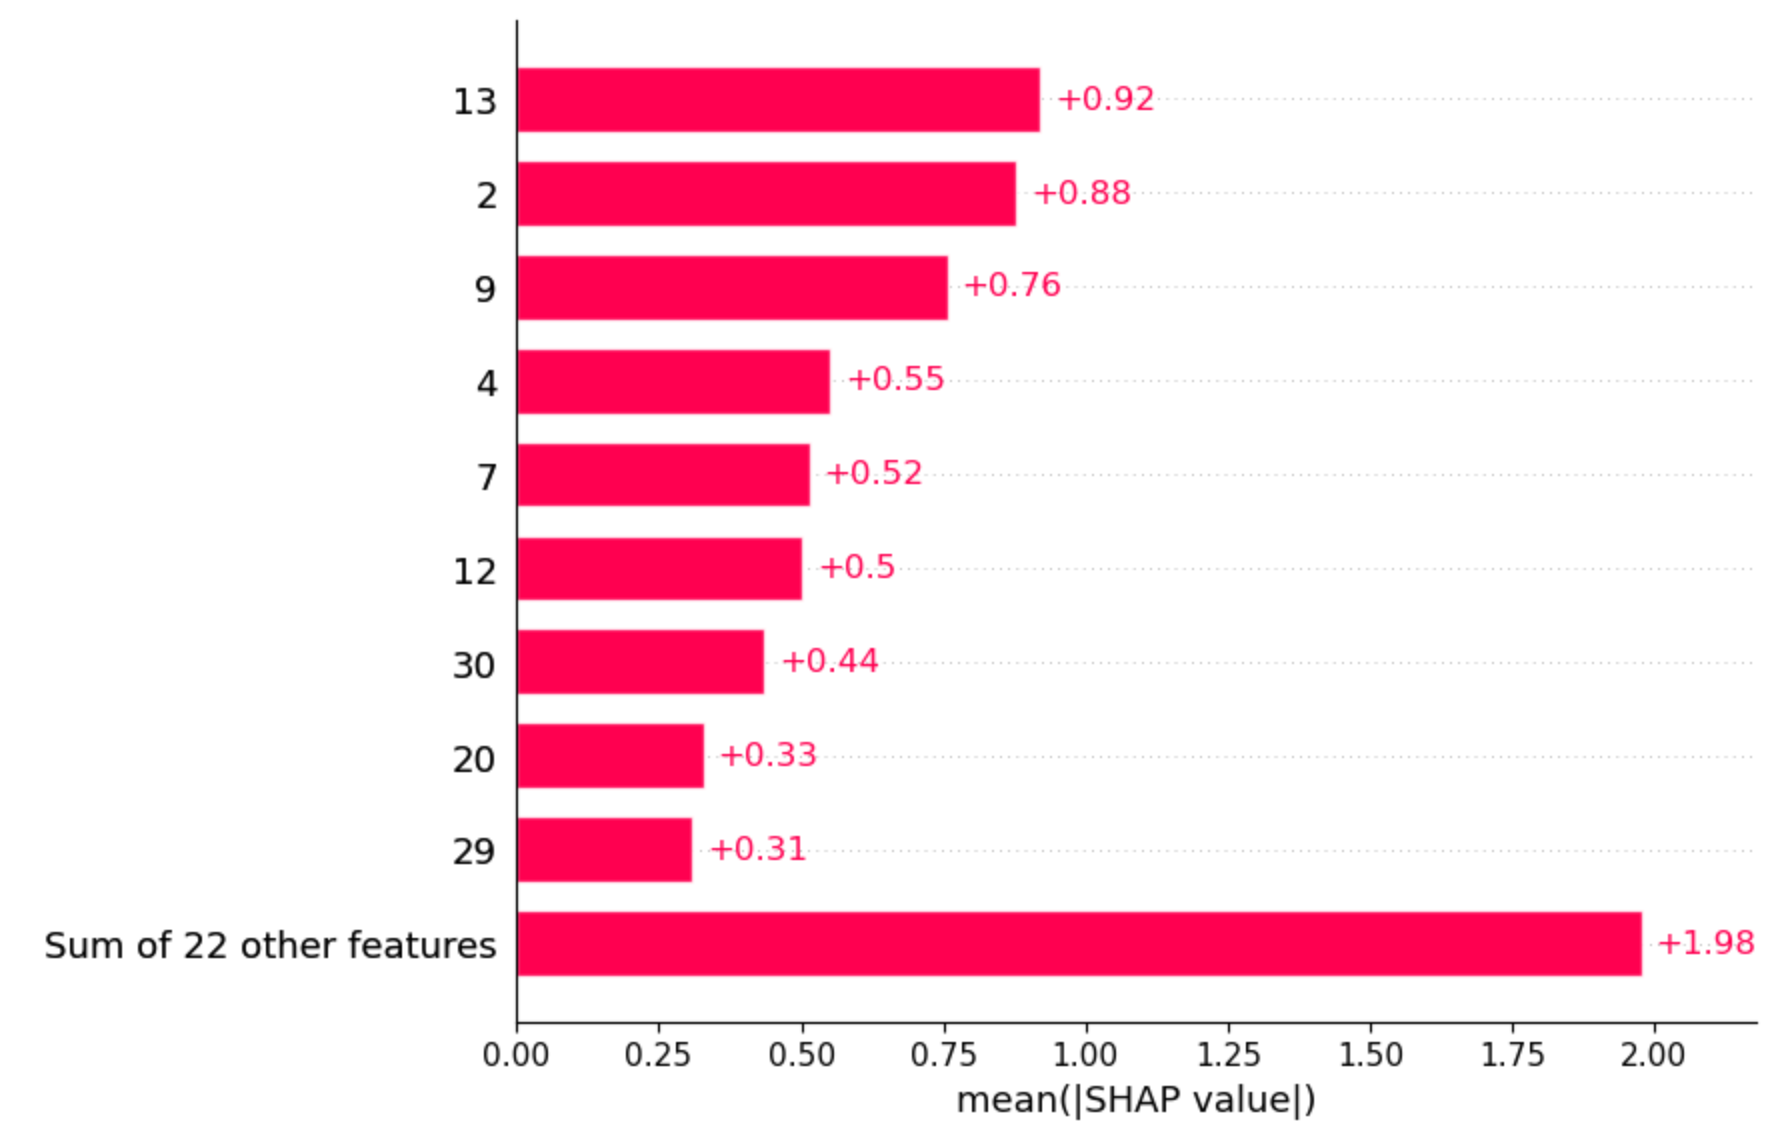
\includegraphics[width=0.8\textwidth]{media/ict/image18}
	\caption*{}
\end{figure}


{\bfseries Fig.2.- Mean SHAP Bar Plot (top pass/fail features)}

\emph{{\bfseries Good/Not Good Analysis}}

Good/not good analysis' s top features are slightly
different. As shown in Figure 3, Course ID plays a major role,
indicating that some courses might be harder or have different grading
standards. Last semester's GPA (29) is a strong predictor of success,
showing that students who performed well previously are likely to
continue doing so. Having a job (5) appears to impact grades, as working
students might struggle with time management and balancing
responsibilities. Accommodation type (10) also matters, suggesting that
living in a dorm, rental, or with family could affect study habits and
comfort. Participation in sports or artistic activities (6) may
influence academic performance, possibly by improving discipline and
time management or taking time away from studying. Father's occupation
(16), Scholarship type (4), and Mother's education level (11) appear to
impact success, possibly affecting academic and financial support.


\begin{figure}[H]
	\centering
	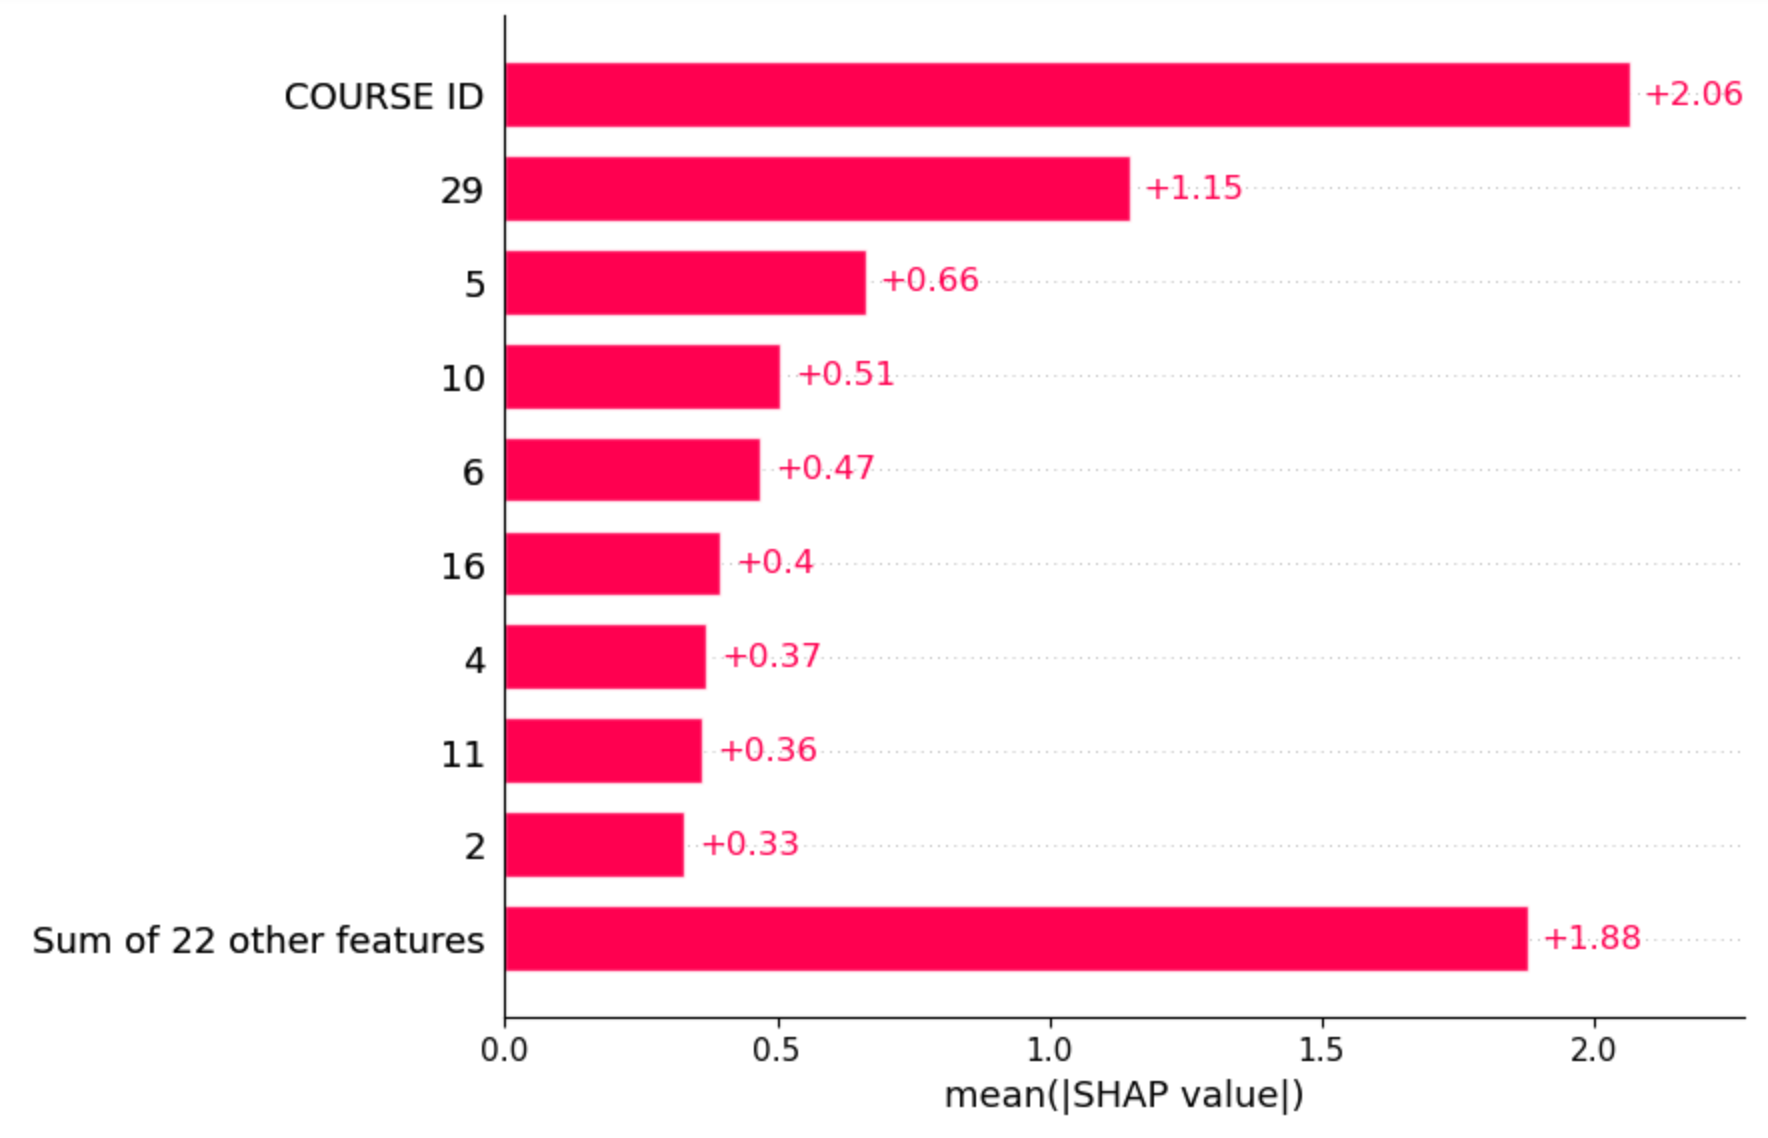
\includegraphics[width=0.8\textwidth]{media/ict/image19}
	\caption*{}
\end{figure}


{\bfseries Fig.3 -Mean SHAP Bar Plot (top good/not good features)}

\emph{{\bfseries Prediction Accuracies}}

In order to predict accuracies 6 different ML models are used. But in
Table 1, only the highest accuracy score among them is written. Table 1
shows the accuracy of different prediction models based on the features
used. When we use all features to predict all grades (A to F), the
accuracy is 36.23\%, which is quite low. Using only the top features for
Pass/Fail prediction, the accuracy slightly improves to 36.30\% when
predicting all grades. However, when we focus on predicting whether a
grade is Good or Not Good, the accuracy increases to 42.32\%, showing
that this classification is a bit easier. When the model predicts only
Pass or Fail using the top Pass/Fail features, the accuracy jumps to
97.43\%, meaning it is very effective at distinguishing between passing
and failing students. Similarly, when predicting Good or Not Good using
the top Good/Not Good features, the accuracy is 80.07\%, which is also
quite high. This suggests that using the right features for a specific
type of prediction greatly improves accuracy, especially for simpler
classifications like Pass/Fail.

{\bfseries Table 2 - Prediction Accuracies}

%% \begin{longtable}[]{@{}
%%   >{\centering\arraybackslash}p{(\linewidth - 4\tabcolsep) * \real{0.3964}}
%%   >{\centering\arraybackslash}p{(\linewidth - 4\tabcolsep) * \real{0.3299}}
%%   >{\centering\arraybackslash}p{(\linewidth - 4\tabcolsep) * \real{0.2737}}@{}}
%% \toprule\noalign{}
%% \endhead
%% \bottomrule\noalign{}
%% \endlastfoot
%% Features & Predict Grade & Accuracy Score \\
%% All & All & 36.23\% \\
%% Top Pass/Fail & All & 36.30\% \\
%% Top Good/Not Good & All & 42.32\% \\
%% Top Pass/Fail & Pass/Fail & 97.43\% \\
%% Top Good/Not Good & Good/Not Good & 80.07\% \\
%% \end{longtable}

Our results show that prior academic performance is a strong indicator
of future success, with last semester's GPA and expected graduation GPA
being the most influential factors in determining whether a student
passes or fails. Additionally, course-related features such as course ID
played a major role in predicting good or not good performance,
suggesting that certain courses may be more challenging than others.
Other significant factors include employment status, accommodation type,
and parental education, indicating that both personal and environmental
conditions affect learning outcomes. The model performed exceptionally
well in pass/fail classification with an accuracy of 97.43\%, while
good/not good classification reached 80.07\%, showing that broad
classifications are easier to predict than detailed grade levels.

{\bfseries Conclusion.} In this study, we explored how different student
characteristics influence performance in e-learning courses using the
XGBoost classifier and SHAP analysis. By focusing on key factors such as
academic history, family background, and educational habits, we aimed to
understand which features have the most impact on predicting student
grades. Our approach allowed us to break down student success into three
categories: predicting exact grades, distinguishing between passing and
failing students, and identifying whether a student performs well or
not. By applying machine learning techniques, we gained valuable
insights into the elements that contribute to academic achievement in
online education.

For future research, using a larger and more diverse dataset could
improve the reliability of predictions and allow for more generalizable
conclusions. Including behavioral data such as student engagement,
online participation, and study patterns could further enhance model
accuracy. Additionally, investigating psychological factors like
motivation and stress levels may provide deeper insights into student
performance.

{\bfseries References}

1. P.Lam J. Lee M. Chan, C. Mcnaught Students' use of elearning
strategies and their perceptions of elearning usefulness//Global
Learn.-\emph{~} 2011. - P.1379--1388

2. H.A.Tanye Quality elearning in distance learning: Benefits and
implications for national elearning policy in Ghana// International
Journal of Multicultural and Multireligious
Understanding.-2017.-Vol.4(3).- P.1-8. DOI
\href{http://dx.doi.org/10.18415/ijmmu.v4i3.73}{10.18415/ijmmu.v4i3.73}

3. F. Concannon, A. Flynn, M. Campbell What campus-based students think
about the quality and benefits of e-learning/ British Journal of
Educational Technology.-2005.-Vol.36(3).-P.501-512

pp.501--512, 2005. DOI
\href{http://dx.doi.org/10.1111/j.1467-8535.2005.00482.x}{10.1111/j.1467-8535.2005.00482.x}

4. E.K.Abed Electronic learning and its benefits in education// Eurasia
Journal of Mathematics, Science and Technology Education. -- 2019.-
Vol.15(3).- P.1-8. DOI 10.29333/ejmste/102668

Malaysian Online Journal of Instructional Technology

ISSN: 1823-1144

Vol.2, No.1, April 2005

Malaysian Online Journal of Instructional Technology

ISSN: 1823-1144

Vol.2, No.1, April 2005

Malaysian Online Journal of Instructional Technology

ISSN: 1823-1144

Vol.2, No.1, April 2005

Malaysian Online Journal of Instructional Technology

ISSN: 1823-1144

Vol.2, No.1, April 200

5. M.S.Bowles Learning to e-learn project: Rediscovering the benefits of
e-learning// Malaysian Online Journal of Instructional
Technology.-2005.-Vol.2(3). -- P.1823--1144

6. M.A. Almaiah, A. Al-Khasawneh, A. Althunibat Exploring the critical
challenges and factors influencing the e-learning system usage during
covid-19 pandemic // Education and Information Technologies.- 2020.-Vol.
25(1). DOI
\href{https://link.springer.com/article/10.1007/s10639-020-10219-y}{10.1007/s10639-020-10219-y}

7. A.M.Maatuk, E.K. Elberkawi, S.Aljawarneh, H.Rashaideh, H. Alharbi The
covid-19 pandemic and e-learning: challenges and opportunities from the
perspective of students and instructors// Journal of Computing in Higher
Education.2022.-Vol.34(1).- P.21-38. DOI
\href{https://doi.org/10.1007/s12528-021-09274-2}{10.1007/s12528-021-09274-2}

8. W.A.Cidral, T.Oliveira, M.D. Felice, M.Aparicio E-learning success
determinants: Brazilian empirical study// Computers and Education.-
2018. -Vol.122.- P.273- 290.

DOI 10.1016/j.compedu.2017.12.001

9. A.Y.Alqahtani, A.A.Rajkhan E-learning critical success factors during
the covid-19 pandemic: A comprehensive analysis of e-learning managerial
perspectives// Education Sciences.-2020.-Vol.10(9):216. DOI
\href{http://dx.doi.org/10.3390/educsci10090216}{10.3390/educsci10090216}

10. D.Al-Fraihat, M.Joy, R.Masa'deh, J.Sinclair, Evaluating e-learning
systems success: An empirical study// Computers in Human
Behavior.-2020.-Vol.102.-P.67-86. DOI 10.1016/j.chb.2019.08.004

11. H.Kauffman A review of predictive factors of student success in and
satisfaction with online learning// Research in Learning
Technology.-2015.-Vol.15.- P.1-15.
DOI~\href{https://doi.org/10.3402/rlt.v23.26507}{10.3402/rlt.v23.26507}

12. A. M. Nortvig, A. K. Petersen, and S. H. Balle, A literature review
of the factors influencing e-learning and blended learning in relation
to learning outcome, student satisfaction and engagement// Electronic
Journal of e-Learning.-2018.-Vol.16(1).-P.46 - 55.

13. N.Yilmaz, B. Sekeroglu Higher Education Students Performance
Evaluation// UCI Machine Learning Repository.-2019 DOI /10.24432/C51G82.

14. Scott M. Lundberg, Su-In Lee Paul G. A unified approach to
interpreting model predictions//31st Conference on Neural Information
Processing Systems (NIPS 2017), Long Beach, CA, USA.-2017.-Vol.25(2).
DOI
\href{http://dx.doi.org/10.48550/arXiv.1705.07874}{10.48550/arXiv.1705.07874}

15. T. Chen, C. Guestrin, ``Xgboost: A scalable tree boosting system//
the 22nd ACM SIGKDD International Conference.2016.- P.785-794. DOI
\href{http://dx.doi.org/10.1145/2939672.2939785}{10.1145/2939672.2939785}

\emph{{\bfseries Information about authors}}

Madeniyetov M. A.- Master's student in Software Engineering at the
School of Information Technology and Engineering, Kazakh-British
Technical University, Almaty, Kazakhstan, e-mail:
\href{mailto:m_madeniyetov@kbtu.kz}{}.

\emph{{\bfseries Сведения об авторе}}

Мәдениетов М.А. - магистрант направления Программная инженерия Школы
информационных технологий и инженерии Казахстанско-Британского
технического университета, Алматы, Казахстан, е -mail:
m\_madeniyetov@kbtu.kz.\